\documentclass[lettersize,journal]{IEEEtran}
\usepackage{amsmath,amsfonts}
\usepackage{algorithmic}
\usepackage{algorithm}
\usepackage{array}
\usepackage[caption=false,font=normalsize,labelfont=sf,textfont=sf]{subfig}
\usepackage{textcomp}
\usepackage{stfloats}
\usepackage{url}
\usepackage{verbatim}
\usepackage{graphicx}
\usepackage{cite}
\usepackage{wasysym}
\usepackage{mathrsfs}



%
% \usepackage{biblatex}
%
% \usepackage[fleqn]{amsmath}
% \usepackage{amssymb}
% \usepackage{graphicx}
% \usepackage{cancel}
% \usepackage{tabularx}
%
% \usepackage{caption}
% % \usepackage{subcaption}
%
% \usepackage{subfig}
% \addbibresource{./citations.bib}
%
% \graphicspath{ {C:/Users/Indy-Windows/Documents/MAE298_Intro_to_PDEs/images/} }
\graphicspath{ {C:/Users/jonat/Documents/MAE298_Intro_to_PDEs/images/} }


\newcommand{\volume}{{\ooalign{\hfil$V$\hfil\cr\kern0.08em--\hfil\cr}}}
%
% \usepackage{hyperref}
% \hypersetup{
% colorlinks=false,
% linkcolor=blue,
% filecolor=magenta,
%     urlcolor=blue,
% }
% \urlstyle{same}
% \setmathfont{XITS Math}
% updated with editorial comments 8/9/2021

\begin{document}

\title{MAE 298 Introduction to PDEs \\ Electrochemical Modeling of Batteries}

\author{Jonathan Dorsey}


% Remember, if you use this you must call \IEEEpubidadjcol in the second
% column for its text to clear the IEEEpubid mark.

\maketitle

% \begin{abstract}
% This
% \end{abstract}

\section{Introduction}
\IEEEPARstart{P}{artial} differential equations (PDEs) provide the mathematical basis for describing many significant scientific phenomena; however, while an important domain of study in its own right, the application and derviation of PDE based models is often more challenging to understand and develop, than merely studying the mathematical formalism behind PDEs. The inherent complexity of deriving and analyzing PDE models when compared to more approachable ODE models can be further exacerbated by systems of coupled equations and/or nonlinear dynamics. For these systems, the derivation and interpretation of the model are often obfuscated by modeling assumptions, domain specific knowledge, and an understanding of how these mechanisms are translated into a PDE formation. In effect, these PDE models compromise higher accuracy and predictability, at the expense of ease of modeling, computational overhead, intuition, and interpreability. \\

An important modern day example can be found in the study of electrochemical battery models, where even simplified electrochemical model consist of a system of partial differential equations, each describing physical laws and constraints which the dynamics of the battery must obey. The objective of this paper is to derive the salient PDEs that define the microscale first principles electrochemical battery model from which we can distill the well known Doyle-Fuller-Newman (DFN) model and a more simplified Single Particle Model (SPM). The intent of this paper is to provide the reader with enough contex that the reader will be able to understand the development of state of the art electrochemical battery modeling from fundamental assumptions to the principle mechanisms at work with this model, to inform how these concepts are translated into the mathematical language of partial differential equations.

\section{Single Particle Model Overview}
For years, the Doyle-Fuller-Newman model has long been held as the gold standard electrochemical battery model and has been used as a benchmark for modeling and the predictive ability of new battery models and techniques. The DFN model describes the first principles dynamics of a battery cell [Fig. \ref{DFN_schematic}], and encapsulates the dynamics of a lithium-ion battery at the continuum-scale. This is accomplished by derving the microscale governing equations and applying volume averages over the models' domain. The primary elements of this model consist of five governing equations for the conservation of mass in homogeneous solid phase, the conservation of charge in homogeneous solid phase, the conservation of mass in homogeneous electrolyte phase, the conservation of charge in the homogeneous electrolyte phase, and finally the transport effects of lithium movement between the solid and electrlye phases, known as the Bulter-Volmer kinetics equation. \\

Unfortunately, derivation of the full DFN model would require investigation into the process of volume averaging which, in and of itself, is an involved procedure. To this end, this paper will endeavour to derive the underlying microscale model, used to develope both SPM and DFN models, with the end goal of translating the microscale model into the SPM formulation which utilizes a reduction of order to simplify the battery model into the two dimensional problem of 1D space and time. SPM along with its' more accurate cousin (the Single Particle Model with Electrolyte Dynamics {SPMe}), take the approach that simplifying the domain which the PDE defines, is an acceptable tradeoff of accuracy for a measurable boost in computational efficiency. As such these models have found growing acceptance in the domain of real-time or near real-time applications such as battery state of charge estimation, which has been dominated by lumped parameter ODE equivalent circuit models (ECM). \\

 The majority of this paper will investigate the process of deriving the microscale governing partial differential equations, from which we can derive the Single Particle battery model. For reference the desired microscale model equations are listed below. Throughout this paper, the reader will see how individual components of physics, chemistry, and thermodynamics are brought together to to derive the following set of partial differential equations.

\begin{figure}
  \centering
  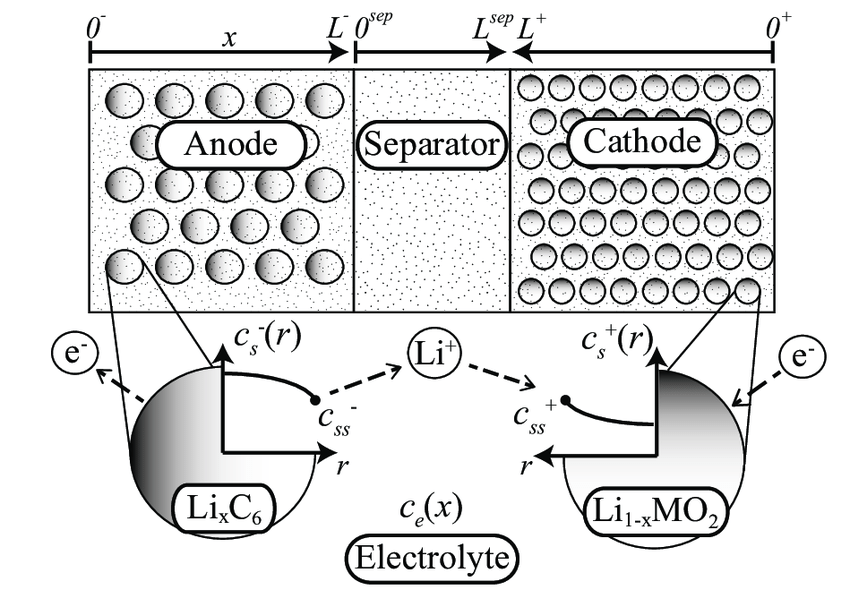
\includegraphics[scale=.25]{DFN}
  \caption{Planar DFN Model Schematic}
  \label{DFN_schematic}
\end{figure}

\begin{equation} \label{COC_s}
\nabla \cdot \mathbf{i}_{s}=\nabla \cdot\left(-\sigma \nabla \phi_{s}\right)=0
\end{equation}

\begin{equation} \label{COM_s}
\frac{\partial c_{s}}{\partial t}=\nabla \cdot\left(D_{s} \nabla c_{s}\right)
\end{equation}

\begin{equation} \label{COM_e}
\frac{\partial c_{e}}{\partial t}=\nabla \cdot\left(D_{e} \nabla c_{e}\right)-\frac{\mathbf{i}_{e} \cdot \nabla t_{+}^{0}}{F}-\nabla \cdot\left(c_{e} \mathbf{v}_{0}\right)
\end{equation}

\begin{equation}\label{COC_e}
\nabla \cdot\left(-\kappa \nabla \phi_{e}-\frac{2 \kappa R T}{F}\left(1+\frac{\partial \ln f_{\pm}}{\partial \ln c_{e}}\right)\left(t_{+}^{0}-1\right) \nabla \ln c_{e}\right)=0
\end{equation}

\begin{equation} \label{lithium_movment}
j=\frac{i_{0}}{F}\left\{\exp \left(\frac{(1-\alpha) F}{R T} \eta\right)-\exp \left(-\frac{\alpha F}{R T} \eta\right)\right\}
\end{equation}

\section{Microscale Model Derivation}

 In the microscale model, the principle mechanisms of operation are evaluated under the assumption of homogeneous solid and electrolyte phases. With these assumptions, the model does not need to account for individual molecular interactions or impurities, as these are assumed to be averaged out to create a homogeneous material that can be directly used to derive and evaluate the governing equations in both the solid and electroyte phases of the battery. \\

 At the microscale, we are interested in deriving the governing equations which are pertainent to the operation of a lithium-ion battery. These governing equations are ...\\

 \begin{enumerate}
   \item Conservation of Mass in homogeneous solid phase
   \item Conservation of Charge in homogeneous solid phase
   \item Conservation of Mass in homogeneous electrolyte
   \item Conservation of Charge in homogeneous electrolyte
   \item Lithium Reaction Kinetics \\
  \end{enumerate}

The two domains that we are interested in solving these equations for are the homogeneous solid which is represented by the battery electrodes, as well as the homogeneous electrolyte which represents the electrically conductive liquid medium inbetween the anode and the cathode. When coupled with the dynamics of lithium transport into the active material of the electrode, these equations will define all of the salient dynamics which a lithium-ion battery will incorporate. We will begin with the conservation of charge in the solid phase.

\subsection{Charge Conservation in Homogeneous Solid}

From physics, we know that electric charge must be conserved in an isolated system. For the purposes of this paper, we will assume that the battery we are modeling constitutes an isolated system that does not interact electrically with its environement. This is a reasonable assumption. Therefore, if the convseration of charge must hold, then it must be true that charge is not created or destroyed inside of the solid electrodes. This is expressed symbolically as the following surface integral of current flux density.

\begin{equation}
 I = - \oiint_S \textbf{i} \cdot d \textbf{S}
\end{equation}

\noindent Where the net current into an arbitary surface \textbf{S} can be written in terms of the surface integral of current density \textbf{i}. Via application of the Divergence Theorem and Conservation of Charge, it can be shown that ...

\begin{equation}
    I = - \iiint_{\volume} (\nabla \cdot \textbf{i})d{\volume} = 0
\end{equation}

\noindent Since we assume charge in the volume of integration must be conservated, and since current is the time rate of change of charge, we can state that the net currrent flow into/out of the volume of integration must be zero.  In this form, we note that since the entire volume integral must equate to zero, the integrand must also be indentically equal to zero.

\begin{equation} \label{con_charg_solid}
    \nabla \cdot \textbf{i} = 0
\end{equation}

While this statement is an accurate formulation of \textbf{conservation of charge}, we would like to formulate this same expressions as a function of electric potential, instead of current density. This can be done by applying the point form of \textbf{Ohm's Law}, namely $\textbf{i} = \sigma\textbf{E}$, where the electric field $\textbf{E} = -\nabla \phi$.
\begin{equation} \label{ohms_law}
  \textbf{i} = -\sigma \nabla \phi
\end{equation}

\noindent By substituting equation (\ref{ohms_law}) into (\ref{con_charg_solid}), we arrive at the final form of the conservation of charge in the electrodes, shown below.
\begin{equation} \label{final_COC_s}
  \nabla \cdot (-\sigma \nabla \phi_s) = 0
\end{equation}

When stated directly, equation (\ref{final_COC_s}) states that the divergence of the conductivity ($\sigma$) weighted gradient of the electrical potential must equal zero for charge to be conserved in the volume of system which we have defined (aka the battery). This expression must hold true for both electrodes of the battery.

\subsection{Mass Conservation in Homogeneous Solid}

Next, the \textbf{conservation of mass} in homogeneous solid (electrodes) is used to capture the dynamics of lithium transport. The principle mechanism here is diffusion. As such, we can model this behavior as a diffusion process via Fick's first law, where the molar flux density \textbf{N} $[mol m^{-2} s^{-1}]$ is related to the gradient of lithium concentration in the solid electrode material, proportional to a material dependent constant of diffusivity D.
\begin{equation}\label{ficks_first}
    \textbf{N} =  -D \nabla c
\end{equation}

While equation (\ref{ficks_first}) encapsulates the mechanism of diffusion of molar lithium as function of the concentration gradient, we would like to express it in terms of the rate of change of the solid phase lithium concentration. To accomplish this, we first need to compute the net molar flux by taking the integral of the net molar flux density over the entire domain boundary.
\begin{equation}\label{flux_divergence}
  j = -\oiint_{S} \textbf{N} \cdot \hat{\textbf{n}}dS
\end{equation}

This provides us with the net molar flux \textbf{j} $ [mol s^{-1}]$, which can rewritten in terms of molar flow rate, where n is the number of moles of lithium ...
\begin{equation}\label{molar_flux}
    j = \frac{dn}{dt}
\end{equation}

Recalling that the definition of molar concentration is the number of moles of a material divided by the total volume it occupies $\left( c = n / \volume \right)$, we can define an infinitesimal mole $dn$ to be computed by integrating each contribution of concentration within a differential volume over the entire volume of the domain and then taking the derivate with respect to time.
\begin{equation}
    n = \iiint_{\volume} cd{\volume}
\end{equation}

\begin{equation}\label{time_rate_of_molar_flux}
  \frac{dn}{dt} = -\frac{d}{dt} \iiint_{\volume} cd{\volume}
\end{equation}

\noindent By substituting equations (\ref{molar_flux}) and (\ref{time_rate_of_molar_flux}) into equation (\ref{flux_divergence}) we arrive at the following statement.
\begin{equation}\label{COM_s_int_form}
  \oiint_S \textbf{N} \cdot \hat{n}dS = -\frac{d}{dt} \iiint_{\volume} c d{\volume}
\end{equation}

This is the integral form of the continuity equation, which relates the molar flux density, from Fick's First Law, to the concentration of lithium in the solid phase of the battery. \\

\noindent This is an important formulation because it provides the link to express the molar flux density in terms of lithium concentration. While initially a rather opaque connection, in the study of electrochemical battery models, the ability to express find desired dynamics as a function of concentration is desirable since many of the quantities we are interested in understanding with this model are defined as a function of concentration. The best example of this being a batteries state of charge (SOC). \\

 As an equation of continuity, equation (\ref{COM_s_int_form}), states that no mass has been created or destroyed inside the domain. This statement can further be used to imply that all mass transfer happens only at the boundaries of the domain. Equation (\ref{COM_s_int_form}) can be further simplified into the more familiar point form of Fick's second law, as shown below.
\begin{equation}
    \frac{\partial c_{S}}{\partial t} = \nabla \cdot \left( D_{S} \nabla c_{s} \right)
\end{equation}

This law states that the total lithium flux density (in a given volume) must be equal to the rate of change of concentration within that volume.


\subsection{Charge Conservation in Homogeneous Electrolyte}

When discussing the conservation of charge inside of the electrolyte phase of the battery, a non-trivial amount of thermodynamics and physical chemistry are required to fully contextualize the principles for deriving the governing equations. \\

This section will endeavour to lay the foundation for the elements of \textbf{Concentrated Solution Theory}, which are required to formulate the basic tenents of charge conservation in non-trivial chemical solutions, such as a batteries electrolyte. \\

\subsubsection{Gibbs Free Energy}
The first construct to be elaborated is that of Gibbs free energy. Simply put, Gibbs Free Energy is total energy required to create the system (with internal energy u), plus the amount which boundary work (pV) required to make room for the system, minus the energy which is obtained from the surrounding environment (TS), which has a temperature of T. Conceptually, the Gibbs free energy is the amount of useful energy which can be harnessed to do work in a system, and is generally written as.

\begin{equation} \label{gibbs_free_energy}
  G = U + p{\volume} - TS
\end{equation}

 The \textbf{free energy} portion of the name, is important because it informs us of how much energy can be extracted from the system, so long as the temperature and pressure are held constant. Additionally, the sign of the Gibbs free energy dictates the direction that a chemical reaction will spontaneously take. \\

 In the context of batteries, Gibbs free energy is used in the formulation of electrochemical potentials, which are discussed below.\\


 \subsubsection{Molarity \& Molality}

 Since an electrolyte is a solution, it can be described as an intensive property via its molarity and molality, depending on which attributes of the solution are of interest. The molarity of a solution is defined to be the number of moles of solute per liter of solution.

\begin{equation}\label{molarity}
    c_i = \frac{n_{solute_i}}{{\volume}_{solution}}
\end{equation}


 \noindent Where as the molality of the solution, is defined to be the total number of moles of solute over the mass of the solvent.

 \begin{equation}\label{molality}
     m_i = \frac{n_{solute_i}}{m_{solvent}}
 \end{equation}

 \subsubsection{Electrochemical Potential}

 Understanding the previous sections is important because it leads to a discussion of electrochemical potentials. Especially in multispecies solutions, the conversion from extensive properties to intensive properties is subtle. In order to properly define these intensive properties, it is neccessary to define partial molar quantities. This can be written using partial derivatives and describes how much the Gibbs free energy (extensive) changes with the addition of only species to the solution. This can be written...

 \begin{equation}\label{electrochemical_potential}
     \bar{\mu} = \left( \frac{\partial G}{\partial n_{i}} \right)_{T,p,n_{j} (j \neq i)}
 \end{equation}

 \noindent where $n_i$ is the number of moles of species $i$, while keeping the temperature, pressure, and moles of other species constant.  Given this definition, note that electrochemical potential is an intensive property which has been normalized via the species mass (in moles).\\

 By evaluating the composition of equation (\ref{gibbs_free_energy}), we can see that Gibbs free energy can be written in terms of internal and external energy components. Therefore it follows that equation (\ref{electrochemical_potential}), which defines the total potential, can be written in terms of internal and external potentials, which is written as.

\begin{equation}
  \bar{\mu_{i}} = \bar{\mu}_{i, internal} + \bar{\mu}_{i, external}
\end{equation}

 In the absence of other potentials and forces from external fields, the effect of chemical and electrochemical potentials can be written as ...
 \begin{equation}\label{total_potential}
   \bar{\mu}_{i} = \mu_{i} + z_i F \phi
 \end{equation}

Where the $z_i$ is the charge number, $F$ is Faraday's constant, and $\phi$ is the local electrostatic potential. The second term of this equation defines the potential associated with the electric field $\phi$. This equation neatly seperates the potential contributions from both chemical and electrical mechanisms. After applying Euler's theorem for homogeneous functions we can show that Gibbs free energy can be neatly written as a function of electrochemical potentials, as shown below.

\begin{equation}
  G(\textbf{n}) = \textbf{n} \cdot \nabla G (\textbf{n}) = \sum_i n_i \frac{\partial G}{\partial n_i}
\end{equation}

\begin{equation}\label{gibbs_summation}
  G = \sum_i n_i \bar{\mu}_i
\end{equation}

\noindent This notion provides a very compact form for expressing the connection between Gibbs free energy and the associated total potentials (chemical \& electrical) that the battery contains.  \\

\subsubsection{Gibbs-Duhem Equation}
The \textbf{Gibbs-Duhem} equation provides an important relationship between electrochemical potentials, which reduces the number of simultaneous equations which we must solve. It's derivation begins with the Gibbs Free Energy as shown below.

\begin{equation}
  G = U + pV - TS
\end{equation}

\begin{equation}
    dG = dU + d(pV) - d(TS)
\end{equation}

\begin{equation}
  = dq + dw + pdV + VdP -TdS - SdT
\end{equation}

\noindent Note that so far, all that has been accomplished has been applying the derivative operator, expanding the expression via the product rule of differentiation, and expanding the interal energy into the equivalent energy of heat and work.  \\

\noindent From thermodynamics of our battery system, we know $dw = -pdV$ and that under the assumption of reversibility $dq = TdS$. After applying these substitutions, we arrive at the simplifed expressions below.

\begin{equation}
  dG = Vdp - SdT
\end{equation}

We can use equations \ref{electrochemical_potential} and \ref{gibbs_summation} to write the previous equation in terms of the total potential.
\begin{equation}
  \sum_{r}^{i=1} n_id\bar{\mu}_i = Vdp - SdT
\end{equation}

\noindent By rearranging the equations we get ...

\begin{equation}
  \sum_{i=1}^{r} n_id\bar{\mu}_i - Vdp + SdT = 0
\end{equation}

\noindent If we assume that pressure and temperature are constant, then derivatives of $p$ and $T$ are both zero. Since we expect to operate the battery in a constant temperature and pressure environment, these are meaningful simplifications which yield the following expression for a system with $i$ chemical species.
\begin{equation}
  \sum_{i=1}^{r} n_id\bar{\mu}_i = 0
\end{equation}

In the special case we are interested in (e.g a binary electrolyte) containing only two species, this equation can be explicitly written as

\begin{equation}\label{gibbs_duhem_eqn}
  n_1 d\bar{\mu}_1 + n_2 d\bar{\mu}_2 = 0
\end{equation}

This is an important equation because it directly governs the relationship between the two potentials. If one is increased, the other must decrease to maintain the equality. We can leverage this relationship to eliminate an equation, in future calculations, since we can write either quantity in terms of the other. This equation can also be written using the concentration of each species by dividing by the total volume.
\begin{equation}
  \sum_{i=1}^{r} c_{i}d\bar{\mu}_i = 0
\end{equation}

\subsubsection{Activity}

Unlike non-ionic solutions, ionic solutions do not distribute their ions randomly, this is because the electrical charge for either a cation or anion are preferentially oriented and attracted to ions of the opposite charge. A consequence of this behavior is that movement of ions in solution are artificially slow, due to the movement of a specific ion also attempting to drag the other ions which are in its immediate neighborhood in the solution. \\

Because of this phenomenon, we define the \textbf{activity} of a species as an effective concentration, which accounts for this descrepency.

\begin{equation}\label{activity}
  a_i = c_i f_i
\end{equation}

In the context of lithium-ion batteries, the concept of activity is important because the transport medium between each electrode is a charge neutral ionic solution, which has a fixed number of positive and negative charge carries, that faciliate transfer of charge inside the battery. Therefore modeling this non-intutiative behavior is an important step in capturing the complete dynamics of mass and charge through the electrolyte. \\

\subsubsection{ Stoichiometric Coefficient $\nu$}
In a balanced chemical equation, the total amount of matter (of each element/molecule) and the total amount of charge are conserved. This fact holds true for electrolytes. In the case of an electrolyte, the solution is comprised of a solute dispursed throughout a solvent such that the overall solution is charge-neutral. An example is shown below.
\begin{equation}
  \mathrm{Na}_{2} \mathrm{SO}_{4} \rightarrow 2 \mathrm{Na}^{+}+\mathrm{SO}_{4}^{2-}
\end{equation}

In this example, the coefficents in from of each ion on the right-hand-side of the equation, are known as \textbf{stoichiometric coefficients}, and are denoted with the symbol $\nu$. In the equation shown above, the stoichiometric coefficents are $\nu_{Na^{+}} = 2$ and $\nu_{SO_{4}^{2-}} = 1$. \\

\subsubsection{ Charge Number}

Similar to the stoichiometric coefficents, the \textbf{charge number} is also displayed in the chemical equation, as the super-script for each compound on the right-hand-side of the the balanced chemical equation. The charge number tells us how many excess electrons or protons exist in each given ionic compound. The charge numbers for the equation above are $z_{Na^{+} = 1}$ and $ z_{SO_{4}^{2-}} = -2 $. The sign of the charge number informs us whether each compound is a cation ($z>0$) or anion ($z < 0 $) \\

\subsubsection{ Charge Neutrality in Binary Electroytes }
For the battery chemistries of interest in this paper, the binary electrolyte comprised of only two species is of particular interest and has useful properties which are very relavent to lithium-ion battery models. Under the constraint of charge-neutrality, we can state that the net charge in the solution must be zero, such that $q = 0$. This can be expressed by using the definition of charge numbers and stoichiometric coefficents described above.

\begin{equation}
  \sum_{i} z_{i} \nu_{i}=0
\end{equation}

For the general case the subscripts indicated whether the charge is from a cation or an anion, or the contributions form the solvent.

\begin{equation}
  z_{+} \nu_{+}+z_{-} \nu_{-}+z_{0} \nu_{0}=0
\end{equation}

However, since the solvents in the electroyte are always charge neutral, we can ommit them from this equation, leavinging the following expression.


\begin{equation}
  z_{+} \nu_{+}+z_{-} \nu_{-}=0
\end{equation}

\begin{equation}
  \frac{c_{+}}{\nu_{+}}=\frac{c_{-}}{\nu_{-}}
\end{equation}

This can be translate from stoichiometric coefficients to the ion concentration of each species, through the fact that we know these quanties must be proportional to each other. Furthermore, the constant of proportionality is the concentation of the entire solution.
\begin{equation}
  c = \frac{c_{+}}{\nu_{+}} = \frac{c_{-}}{\nu_{-}}
\end{equation}

We can make use of this attribute and rewrite the charge neutrality equation in terms of species concentrations as follows.
\begin{equation}
  \sum_{i} z_i c_i = 0
\end{equation}

Where $ i=2$ for our use-case of a binary electrolyte. This expression will be useful later when deriving the conservation of charge in an electrolyte. \\

\subsubsection{ Current Flow in Electrolyte}

Current flow inside of the electrolyte is comprised movement by both cations and anions. Therefore the total current flow inside of the electrolyte is given by

\begin{equation}
  i = i_{+} + i_{-}
\end{equation}

The next step is try write these ionic currents in terms of flux density or species concentrations so that they can be written in standard form later. This is accomplished by accounting for the amount of charge per second (for both cations and anions), due to the respective flux.

\begin{equation}
    i_+ =  z_+ FN_+ = z_{+}Fc_{+}\nu_{+}
\end{equation}

\begin{equation}
  i_- =  z_- FN_- = z_{-}Fc_{-}\nu_{-}
\end{equation}

Upon reflection, we can see that the product of charge number, Faraday's constant, and flux density, is the eletrical current produced for the given charge type (positive/negative). Therefore, we can compactly express this equation using the following summation notion.

\begin{equation}
  i = z_{+}Fc_{+}\nu_{+} + z_- FN_-
\end{equation}

\begin{equation}
  = F\sum_{i}z_{i}N_{i}
\end{equation}

\subsubsection{ Deriving Conservation of Charge}

To begin this derivation, we can start off with the general expression for the conersation of mass at any point in a solution.

\begin{equation}
  \frac{\partial c_{i}}{\partial t}=-\nabla \cdot \mathbf{N}_{i}+R_{i}
\end{equation}

This version of Fick's Law states that the time rate of change on the concentration for species $i$ is related to the negative flux density gradient of that species as well as any contribution due to the rate of generation of species $i$, via term $R_{i}$.

\begin{equation}
  F \frac{\partial z_{i} c_{i}}{\partial t}=-\nabla \cdot\left(z_{i} F \mathbf{N}_{i}\right)+z_{i} F R_{i}
\end{equation}

Via algebra, we can multiply each side of the equation by $z_{i}F$ to get,

\begin{equation}
  \frac{\partial}{\partial t} F \sum_{i} z_{i} c_{i}=-\nabla \cdot\left(F \sum_{i} z_{i} \mathbf{N}_{i}\right)+F \sum_{i} z_{i} R_{i}
\end{equation}

Since the previous equation was written only with respect to a single species in the equation, we need to sum the same equation over each species resulting in the following...

\begin{equation}
  \frac{\partial}{\partial t} F \sum_{i} z_{i} c_{i}=-\nabla \cdot\left(F \sum_{i} z_{i} \mathbf{N}_{i}\right)
\end{equation}

As mentioned in the previous section about charge neutrality, we can see show that the our previous equation that the summation $\sum_{i}z_{i}c_{i}$ must be identically equation to zero since, the overall charge of the electrolyte is zero. We can also that the term $F\sum_{i}z_{i}N_{i}$ matches our previous definition for current shown above. By substituting these terms into the previous expression we arrive at the following equation.

\begin{equation}
  \nabla \cdot \mathbf{i}=0
\end{equation}

This equation is the differential form for the conservation of charge inside the electrolyte, stating that charge and not be created or destroyed.

\subsection{Mass Conservation in Homogeneous Electrolyte}
Similar to how we have conserved mass inside of the electrodes, conservation of mass must also hold inside of the electrolyte. This section provides all of the groundwork required to develope this physical law as it pertains to our battery chemistry. \\

\subsubsection{Maxwell-Stefan Relationship}
This section lays the mathematical groundwork for the interaction of particles of differing species and the net force associated with these collisions. By applying the conservation of momentum, we can define the following expression for using average species velocities, of a two species mixture.

\begin{equation}
  m_{1} \mathbf{v}_{m_{1}}+m_{2} \mathbf{v}_{m_{2}}=m_{1} \mathbf{v}_{m_{1}}^{\prime}+m_{2} \mathbf{v}_{m_{2}}^{\prime}
\end{equation}

Given that the change in momentum for a single species can be written as...

\begin{equation}
  \Delta\left(m_{1} \mathbf{v}_{m_{1}}\right)=m_{1}\left(\mathbf{v}_{m_{1}}-\mathbf{v}_{m_{1}}^{\prime}\right)
\end{equation}

We can isolate the post-collision velocity of species one, as follows.

\begin{equation}
  \mathbf{v}_{1}^{\prime}=\frac{m_{1} \mathbf{v}_{1}+m_{2} \mathbf{v}_{2}}{m_{1}+m_{2}}
\end{equation}

These two previous expressions can be combined to form the following equation.

\begin{equation}
  \begin{aligned}
  \Delta\left(m_{1} \mathbf{v}_{1}\right) &=m_{1}\left(\mathbf{v}_{1}-\mathbf{v}_{1}^{\prime}\right) \\
  &=m_{1}\left(\mathbf{v}_{1}-\frac{m_{1} \mathbf{v}_{1}+m_{2} \mathbf{v}_{2}}{m_{1}+m_{2}}\right)
  \end{aligned}
\end{equation}

Which can be simplified to...

\begin{equation}
  =\frac{m_{1} m_{2}}{m_{1}+m_{2}}\left(\mathbf{v}_{1}-\mathbf{v}_{2}\right)
\end{equation}

\subsubsection{Momentum Charnge Rate}
Now the task is to relate the change of momentum equation (on a mass basis) to the equivalent form on a species concentration basis. Generally speaking we can state that as the concentions of either species in a two species mixture increase the change in momentum should increase propotionally. Putting this intuition into math, we arrive at the following statement of proportionality.

\begin{equation}
  \left(\frac{\mathrm{dp}}{\mathrm{d} t}\right)_{V}^{\text {species- }} \propto c_{1} c_{2}\left(\mathbf{v}_{1}-\mathbf{v}_{2}\right)
\end{equation}

From this statement, we can use the definition of the mole fraction $x_i = n_i /n$, where $n_i$ is the number of moles of a given species and $n$ is the total number of moles in the system. This defines the following constraint that $x_1 + x_2 = 1$ for a binary species and in general form can be written as $\sum_i x_i = 1$. Furthermore, we can define a quantity called the total concentration, such that.

\begin{equation}
  C_{T}=\sum_{i} c_{i}
\end{equation}

Where concentration is defined as $c = n/ \volume$.  From this relationship we can show that.

\begin{equation}
  x_{i}=\frac{n_{i}}{n}=\frac{n_{i} / \volume}{n / \volume}=\frac{c_{i}}{c_{T}}
\end{equation}

Which can be substituted directly into the change of momentum equation to produce...

\begin{equation}
  \left(\frac{\mathrm{d} \mathrm{p}}{\mathrm{d} t}\right)_{\volume}^{\text {species- }} \propto x_{1} x_{2}\left(\mathrm{v}_{1}-\mathrm{v}_{2}\right)
\end{equation}

From undergraduate physics, Newton's Second law states that force is equivalent to the time rate of change of momentum, leading us to the following statement.

\begin{equation}
  \mathrm{F}_{1, \mathrm{~\volume}} \propto x_{1} x_{2}\left(\mathrm{v}_{1}-\mathrm{v}_{2}\right)
\end{equation}

In order to turn this proportionality into an equality we must define a constant of proportionality. Given that this equation relates forves to relative velocities, it would be natural to define a type of coefficient of friction, $K_{ij}$. \\

However, note that the friction coefficient itself would not be a constant since it would be composed in terms of molar fractions and hence the concentration of the species in the system.

\begin{equation}
  K_{i j} \propto x_{1}x_{2}
\end{equation}

It turns out that the resulting equality has been defined in terms of the Maxwell-Stefan diffusivity $\mathscr{D}$, and the surrounding pressure.

\begin{equation}
  \mathscr{D}_{i j}=\frac{x_{i} x_{j}}{K_{i j}} p
\end{equation}

By applying the ideal gas law and substituting the concentration form of the mole fraction developed earlier, we get.

\begin{equation}
  K_{i j}=\frac{R T c_{i} c_{j}}{c_{T} \mathscr{D}_{i j}}
\end{equation}

After developing these expressions, we can subsitute them back into the original equation for the force acting on species one.

\begin{equation}\label{friction_force_1}
  \mathbf{F}_{1, V}=\frac{R T c_{1} c_{2}}{c_{T} \mathscr{D}_{12}}\left(\mathbf{v}_{1}-\mathbf{v}_{2}\right)
\end{equation}

Now that we have an expression for the force acting on a species , we can begin to make the connections between forces and the electrochemical potential for charged species. \\


\subsubsection{Multicomponent Diffusion Equation}

We know from physics that can write an arbitrary force as the negative gradient of a driving potential function. In the study of our battery, this potential function is the Gibbs free energy developed previously. Furthermore, we can use the chain rule of calculus, to write the gradient of Gibbs free energy in terms of the gradient of the electrochemical potential and the rate of change of Gibbs free energy with respect to electrochemical potential. By using indentities for Gibbs free energy developed ealier, we can show that.

\begin{equation}
  \mathrm{F}_{1}=-\nabla G_{1}=-\frac{\partial G_{1}}{\partial \mu_{1}} \nabla \bar{\mu}_{1}=-n_{1} \nabla \bar{\mu}_{1}
\end{equation}

When this expression is normalized by volume, we can write the force of the particle in terms of species concentration.

\begin{equation}\label{friction_force_2}
  \mathrm{F}_{1, \volume}=\frac{\mathrm{F}_{1}}{\volume}=-\frac{n_{1}}{\volume} \nabla \bar{\mu}_{1}=-c_{1} \nabla \bar{\mu}_{1}
\end{equation}

We can then equate equation (\ref{friction_force_1}) for the net force of a multi-species solution to equation (\ref{friction_force_2}) defining the net force as a function of electrochemical potential gradients to get the following equation.

\begin{equation}
  c_{1} \nabla \mu_{1}=R T \frac{c_{1} c_{2}}{c_{T} \mathscr{D}_{12}}\left(\mathbf{v}_{2}-\mathbf{v}_{1}\right)
\end{equation}

\begin{equation}
  c_{i} \nabla \mu_{i}=R T \sum_{j} \frac{c_{i} c_{j}}{c_{T} \mathscr{D}_{i j}}\left(\mathbf{v}_{j}-\mathbf{v}_{i}\right)=\sum_{j} K_{i j}\left(\mathbf{v}_{j}-\mathbf{v}_{i}\right)
\end{equation}

After summing over all species in the mixture, we arrive at the following final equation.

\begin{equation}\label{mulit_component_mixture_friction}
  \sum_{i} c_{i} \nabla \mu_{i}=\sum_{i} \sum_{j} K_{i j}\left(\mathbf{v}_{j}-\mathbf{v}_{i}\right)
\end{equation}

The significance of this equation is that it produces a basis for analysis using quanitities available at the macroscopic level, and will be used later in the derivation of mass conservation in electrolyte.\\

\subsubsection{Concentrated Binary Electrolyte Theory: Ion Fluxes}

The objective of this next section is to define the ionic flux density, $N_{\pm}$. However, due to the chemical nature of electrolytes, the physical chemistry associated with an excess of charge in the solution, proves to be significantly more challenging and complex than deriving conservation of mass in a non-ionic medium. The primary reasons for this are generally caused by, chemical potentials, average diffusivity, and the transference number associated with electrolyte dynamics. Each of these topics will be addressed in turn before we arrive at an acceptable expression for the flux-density, of lithium in the electrolyte phase. \\

Previously, we developed expressions for the electrochemical potentials for each species; however, for this analysis we would like to define a chemical potential for the electrolyte as a whole. This can be accomplished by defining the eletrolyte chemical potential as the stoichiometry weighted sum of the positive and negative electrochemical potentials, as follows.

\begin{equation}\label{electro_chem_potential}
\mu_{e}=v_{+} \bar{\mu}_{+}+v_{-} \bar{\mu}_{-}
\end{equation}

This expression can then be expanded by substituting equation (\ref{total_potential}), which expands the electrochemical potential into its chemical and electrical potentials.


\begin{equation}
\begin{aligned}
\mu_{e} &=v_{+} \bar{\mu}_{+}+v_{-} \bar{\mu}_{-} \\
&=v_{+}\left(\mu_{+}+z_{+} F \phi\right)+v_{-}\left(\mu_{-}+z_{-} F \phi\right) \\
&=v_{+} \mu_{+}+v_{-} \mu_{-}+\left(v_{+} z_{+}+v_{-} z_{-}\right) F \phi \\
&=v_{+} \mu_{+}+v_{-} \mu_{-}
\end{aligned}
\end{equation}

Note that in this expansion, the electrical potential will cancel out, due to charge neutrality in our electrolyte. This means that the resulting potential is not a electrochemical potential, but only a chemical potential as the net electrical effect is zero. Once we have the expression for the electrolyte chemical potential, we can find its gradient as follows.

\begin{equation}\label{eletrolyte_chem_pot_grad}
\nabla \mu_{e}=\nu_{+} \nabla \bar{\mu}_{+}+\nu_{-} \nabla \bar{\mu}_{-}
\end{equation}


The reason for computing the gradient of the electrolyte chemical potential is to develop an expression which can be substituted in for $\nabla \mu_i$ in equation (\ref{mulit_component_mixture_friction}). Note that, as a reduction of notion, $c_{\pm} = c \nu_{\pm}$ as shown below


\begin{equation}\label{stoich_concentration_pos}
c v_{+} \nabla \bar{\mu}_{+}=c_{+} \nabla \bar{\mu}_{+}
\end{equation}
\begin{equation}\label{stoich_concentration_neg}
   c v_{-} \nabla \bar{\mu}_{-}=c_{-} \nabla \bar{\mu}_{-}
\end{equation}

By substituting the definition of the chemical potential gradient in equation (\ref{eletrolyte_chem_pot_grad}), and the expressions we have for $c_{\pm}$ shown above, into equation (\ref{mulit_component_mixture_friction}), we arrive at the following two equations.

\begin{equation}
\begin{array}{l}
c_{+} \nabla \bar{\mu}_{+}=K_{+0}\left(\mathbf{v}_{0}-\mathbf{v}_{+}\right)+K_{+-}\left(\mathbf{v}_{-}-\mathbf{v}_{+}\right) \\
c_{-} \nabla \bar{\mu}_{-}=K_{-0}\left(\mathbf{v}_{0}-\mathbf{v}_{-}\right)+K_{-+}\left(\mathbf{v}_{+}-\mathbf{v}_{-}\right)
\end{array}
\end{equation}

After collecting like terms and canceling where valid, this equation can be written as ...

\begin{equation}
c \nabla \mu_{e}= K_{0+}\left(\mathbf{v}_{0}-\mathbf{v}_{+}\right)+K_{0-}\left(\mathbf{v}_{0}-\mathbf{v}_{-}\right) .
\end{equation}

Which will be used in subsequent part of the flux-density derivation. \\

The second component which we would like to define for the electrolyte as a whole is the diffusion coeffient. To accomplish this, we would like to combine the effects of diffusion from both ionic species in the electrolyte. As with the chemical potential of the electrolyte, the diffusion coefficent will be defined as the stoichiometric weighted average of the diffusion coefficient for both of its constitute species. However, unlike chemical potentials, diffusivity adds reciprocally.

\begin{equation}
\frac{v}{\mathscr{D}}=\frac{v_{+}}{\mathscr{D}_{0}+}+\frac{v_{-}}{\mathscr{D}_{0}-}
\end{equation}

By solving for the diffusivity $\mathscr{D}$ and multiplying by the concetration, as well as applying simplification from equations (\ref{stoich_concentration_pos}) \& (\ref{stoich_concentration_neg}) we obtain...

\begin{equation}
\mathscr{D}=\frac{\nu C}{\frac{C_{+}}{\mathscr{D}_{0+}}+\frac{C_{-}}{\mathscr{D}_{0-}}}
\end{equation}

If we further multiple this expressions by $\frac{RTC_0}{C_T}$ over itself, we have only multiplied by unity and not changed the value of the expressions; however, after applying this transformation, this equation can be written in terms of the Maxwell-Stefan friction coeffiecients derived previously.

\begin{equation}
\mathscr{D}=\frac{v R T c_{0} c}{c_{T}\left(K_{0+}+K_{0-}\right)}
\end{equation}

The third and final component required to define the flux-density, is the transference numbers of the electrolyte. As mentioned previously the ionic nature of the electrolyte has the consequence of incorporating several non-intuitive chemistry tid-bits which require a more subtle analysis. \\

In simple terms the transference number represents the portion of the ionic current which is being carried by a specific species when there exists no gradient in the chemical potential. Intuitiatively, it should make sense the transference number is propotional to amount of friction the ion will encounter, as such we can define this proportionality for both positive and negative species of the electrolyte.


\begin{equation}
t_{+}^{0} \propto K_{0-} \quad \text { and } \quad t_{-}^{0} \propto K_{0+}
\end{equation}

In fact, for a binary electrolyte, we know that the total transference must be equal to unity, since either the positive or negative ionic current flow must be responsible for the net current. Given the previous proportionality, and the constraint of a binary electrolyte medium, we can determine the constant of proportionality directly, which yields the following result.

\begin{equation}\label{transference_num_def}
t_{+}^{0}=\frac{K_{0-}}{K_{0-}+K_{0+}} \quad \text { and } \quad t_{-}^{0}=\frac{K_{0+}}{K_{0-}+K_{0+}} \\
\end{equation}

In order to drastically simplify the derivation of this section, instead of deriving expression for flux-density in the electrolyte phase directly, we direclty jump to the intermediate form of flux-density and proceed to massage it into its final form. We first begin with a more general definition of flux-density as a function of species concentrations and average species velocities.

\begin{equation}
  \textbf{N}_i = c_{i} \textbf{v}_i \quad \text{    where } i = \pm
\end{equation}

The intuition behind this expression is that the flux-density will change propotionally to the average velocity of a species and as a function of the concentration of the species, traversing into the boundary of our domain. \\

As it turns out, we can write expand this general definition into terms which we have already developed. As shown below for $i = \pm$.

\begin{equation}\label{flux_density}
    \mathbf{N}_{i} ={-\frac{v_{i} \mathscr{D}}{v R T} \frac{c_{T}}{c_{0}}} {\nabla \mu_{e}}+{\frac{\mathbf{i} t_{i}^{0}}{z_{i} F}}+{c_{i} \mathbf{v}_{0}}
\end{equation}

However, even in this form, for this equation to be of use, we still need to translate the term for the gradient of the chemical potential into macroscopic quantities such as concentrations...etc. \\

Note that we can expand $\nabla \mu_e$ via the chain rule of calculus, such that it is written in terms of concentration gradients. And furthermore, we can apply the chain rule again for the partial term to express it in terms of the molality of the electrolyte. These operations are written as follows.

\begin{equation}
  \nabla \mu_e = \frac{\partial{\mu_e}}{\partial{c}} \nabla c
\end{equation}

\begin{equation}\label{change_of_variable}
\frac{\partial \mu_{e}}{\partial c}=\frac{\partial \mu_{e}}{\partial \ln m} \frac{\partial \ln m}{\partial c} \\
\end{equation}

The inclusion of the natural-log, in the previous expression, is merely a build-in substitution which will have the effect of simplifying the notion of future steps. \\

However, even with these expansions and change of variables, we have not been able to eliminate ${\mu_e}$ from equation (\ref{change_of_variable}). To accomplish this, we need to derive an alternate expression for the electrochemical potential $\mu$, in terms of absolute activity $\lambda$ and the modal activity coefficent $\gamma$. By definition these are given as...

\begin{equation}
\mu_{i}=R T \ln \left(\lambda_{i}\right)
\end{equation}
\begin{equation}
\lambda_{i}=m_{i} \gamma_{i} \lambda_{i}^{\ominus}
\end{equation}


We can substitute these definitions into the expression for chemical potential of the electrolyte ($\mu_{e}=v_{+} \mu_{+}+v_{-} \mu_{-} $), and simplify to get the following expression.

\begin{equation}
\begin{aligned}
\mu_{e}= v R T\left(\ln m+\ln \gamma_{\pm}\right)+ \cdots \\
v_{+} R T \ln \left(v_{+} \lambda_{+}^{\ominus}\right)+ \cdots \\
v_{-} R T \ln \left(v_{-} \lambda_{-}^{\ominus}\right)
\end{aligned}
\end{equation}


Now that we have an expression for $\mu_e$ in terms of meaningful macroscopic quantities, we can take its derivative with respect to natural-log of the molality, resulting in the following expression.
\begin{equation}\label{chemical_pot_substitute}
\frac{\partial \mu_{e}}{\partial \ln m}=v R T\left(1+\frac{\partial \ln \gamma_{\pm}}{\partial \ln m}\right)
\end{equation}


As we did with the first term of equation (\ref{change_of_variable}), we now wish to solve for the second term of that equation and find a valid substitution which will rewrite this term as a function of concentration. The substitutions and simplifications necessary to complete these are shown below.

\begin{equation}
m=\frac{m_{+}}{v_{+}}=\frac{c_{+}}{v_{+} c_{0} M_{0}}=\frac{c}{c_{0} M_{0}}
\end{equation}


\begin{equation}
\ln m=\ln c-\ln c_{0}-\ln M_{0}
\end{equation}

\begin{equation}
\frac{\partial \ln m}{\partial \ln c}=1-\frac{\partial \ln c_{0}}{\partial \ln c}
\end{equation}

\begin{equation}\label{concentation_subsitute}
\frac{\partial \ln m}{\partial c}=\frac{1}{c}\left(1-\frac{\partial \ln c_{0}}{\partial \ln c}\right)
\end{equation}

By substituting equations (\ref{chemical_pot_substitute}) and (\ref{concentation_subsitute}) into equation (\ref{change_of_variable}), we can rewrite $\nabla \mu_e$ in its final form as ...

\begin{equation}
\nabla \mu_{e}=\frac{v R T}{c}\left(1+\frac{\mathrm{d} \ln \gamma_{\pm}}{\mathrm{d} \ln m}\right)\left(1-\frac{\mathrm{d} \ln c_{0}}{\mathrm{~d} \ln c}\right) \nabla c
\end{equation}


Now that we have an expression for the $\nabla \mu_e$ we can apply it to our equation for the flux-density which is shown below.

\begin{equation}
\mathbf{N}_{+}=-\frac{v_{+} \mathscr{D}}{v R T} \frac{c_{T}}{c_{0}} c \nabla \mu_{e}+\frac{\mathbf{i} t_{+}^{0}}{z_{+} F}+c_{+} \mathbf{v}_{0}
\end{equation}

But before we do, we can clean up the notion of the flux-density by applying the following substitution.
\begin{equation}
D=\mathscr{D} \frac{c_{T}}{c_{0}}\left(1+\frac{\mathrm{d} \ln \gamma_{\pm}}{\mathrm{d} \ln m}\right)
\end{equation}

This resultings in the final form of the flux-density.

\begin{equation}
\mathbf{N}_{+}=-v_{+} D\left(1-\frac{\mathrm{d} \ln c_{0}}{\mathrm{~d} \ln c}\right) \nabla c+\frac{\mathbf{i} t_{+}^{0}}{z_{+} F}+c_{+} \mathbf{v}_{0}
\end{equation}

With this sorted, we can plug it into the diffusion equation

\begin{equation}
\frac{\partial c_{+}}{\partial t}=-\nabla \cdot \mathbf{N}_{+}
\end{equation}



Which results in the following partial differential equation that enforces mass conservation inside of the electrolyte.



\begin{equation}
  \frac{\partial c}{\partial t}=\nabla \cdot\left[D\left(1-\frac{\mathrm{d} \ln c_{0}}{\mathrm{~d} \ln c}\right) \nabla c\right]-\frac{\mathbf{i} \cdot \nabla t_{+}^{0}}{z_{+} v_{+} F}-\nabla \cdot\left(c \mathbf{v}_{0}\right)
\end{equation}

\subsection{Concentrated Solution Theory: Electrolyte Conservation}

This section focuses on the conservation of charge inside of the binary electrolyte of the battery. This analysis will result in the derivation of the following equation.

\begin{equation}
\mathbf{i}=-\kappa \nabla \phi-\frac{\kappa}{F}\left(\frac{s_{+}}{n \nu_{+}}+\frac{t_{+}^{0}}{z_{+} \nu_{+}}-\frac{s_{0} c}{n c_{0}}\right) \nabla \mu_{e}
\end{equation}


However, before starting, now is the perfect time to cover the chemical equation at play and define notion which will be helpful in future steps. Recall that a balanced chemical equation must not only balance, quantity of each molecule/element, but it must also balance the total amount of electrical charge on each side of the reaction. For our usecase of lithium-ion batteries a typical equation would follow the same general structure as the following equation.
\begin{equation}
\mathrm{M}+\mathrm{Li}^{+}+e^{-} \rightleftharpoons \mathrm{LiM}
\end{equation}

This can be written in an equivalent but more useful form as...
\begin{equation}\label{lithium_ion_reaction_balanced}
\mathrm{LiM}-\mathrm{M}-\mathrm{Li}^{+} \rightleftharpoons e^{-}
\end{equation}

This equation represents the interaction of lithium and some arbitrary metal oxide that which forms the active electrode material, as well as producing excess electrons. From basic principles of physics, we assume that the energy of this reaction must be conserved. Because of this fact, the Gibbs free energy of the LHS of equation (\ref{lithium_ion_reaction_balanced}), must be equal to the electical energy of the electons produced on the RHS of the equation. Symbolically, we can use summation notion to express this as follows.

\begin{equation}
  \sum{G} = \sum{E(e)}
\end{equation}

From previous work, we can write the Gibbs free energy and the energy due to the local electrostatic potential as follows.

\begin{equation}
\sum_{i} s_{i} \bar{\mu}_{i}=-n F \phi
\end{equation}

Where the term $s_i$ represent the number of moles of each component of our chemical equation when written in the form of equation (\ref{lithium_ion_reaction_balanced}). This equation can easily be utilized to compute the relationship between the electrochemical and electrostatic potential gradients.

\begin{equation}\label{COE}
\sum_{i} s_{i} \nabla \bar{\mu}_{i}=-n F \nabla \phi
\end{equation}

By application of the Gibbs-Duhem relationship from equation (\ref{gibbs_duhem_eqn}), and accounting for the change from moles to concentration, we write the following expression for the electrolyte.

\begin{equation}
c_{+} \nabla \bar{\mu}_{+}+c_{-} \nabla \bar{\mu}_{-}+c_{0} \nabla \bar{\mu}_{0}=0
\end{equation}

This expression encapsulates the positive, negative, and neutral components of the electrolyte solution, such that $i = +, -, 0$. Thus far, we have only encountered expressions for positive and negative electrochemical potentials but nothing for the neutral case. Thankfully, by leveraging the Gibbs-Duhem equation, we can solve for the gradient of the $0th$ electrochemical potential.

\begin{equation}
\begin{aligned}
\nabla \bar{\mu}_{0} &=-\frac{1}{c_{0}}\left(c_{+} \nabla \bar{\mu}_{+}+c_{-} \nabla \bar{\mu}_{-}\right) \\
&=-\frac{c}{c_{0}}\left(\nu_{+} \nabla \bar{\mu}_{+}+\nu_{-} \nabla \bar{\mu}_{-}\right) \\
&=-\frac{c}{c_{0}} \nabla \mu_{e}
\end{aligned}
\end{equation}

\noindent Via direct substitution of this result into equation (\ref{COE}), it becomes.

\begin{equation}
s_{+} \nabla \bar{\mu}_{+}+s_{-} \nabla \bar{\mu}_{-}-s_{0} \frac{c}{c_{0}} \nabla \mu_{e}=-n F \nabla \phi
\end{equation}

\noindent From the balanced chemical equation, we can write.

\begin{equation}
s_{+} z_{+}+s_{-} z_{-} =-n
\end{equation}

\noindent From this expression we can solve for $s_{-} $ to arrive at the following equation.
\begin{equation}\label{signed_stoich_coef}
    s_{-} =-\left(\frac{z_{+}}{z_{-}} s_{+}+\frac{n}{z_{-}}\right)
\end{equation}

\noindent This expression for $s_{-} $ can be substitute it into the LHS of the conservation of energy equation which we have developed earlier, to yield.

\begin{equation}
{s_{+} \nabla \bar{\mu}_{+}-\left(\frac{z_{+}}{z_{-}} s_{+}+\frac{n}{z_{-}}\right) \nabla \bar{\mu}_{-}}-s_{0} \frac{c}{c_{0}} \nabla \mu_{e}=-n F \nabla \phi
\end{equation}

\noindent After a significant amount of algrebraic rework, we can rewrite the previous equation without the need to reference the positive eletrode electrochemical potential gradient as.
\begin{equation}\label{grad_mu_e_n_grad_mu_n}
\left(\frac{s_{+}}{n v_{+}}-\frac{s_{0} c}{n c_{0}}\right) \nabla \mu_{e}-\frac{1}{z_{-}} \nabla \bar{\mu}_{-}=-F \nabla \phi
\end{equation}

\noindent However, we would still like to express this equation solely in terms of $\nabla \mu_{e}$. To accomplish this, recall via the Maxell-Stefan equation, that we can write the gradient in electrochemical potential as a function of Maxwel-Stefan friction coefficients.
\begin{equation}\label{max_n_stefy}
c_{-} \nabla \bar{\mu}_{-}=K_{0-}\left(\mathbf{v}_{0}-\mathbf{v}_{-}\right)+K_{+-}\left(\mathbf{v}_{+}-\mathbf{v}_{-}\right)
\end{equation}

We can furthermore, use the equation for flux-density equation (\ref{flux_density}) and rearrange it such that...

\begin{equation}\label{flux_density}
c_{i}\left(\mathbf{v}_{i}-\mathbf{v}_{0}\right) =-\frac{v_{i} \mathscr{D}}{v R T} \frac{c_{T}}{c_{0}} \nabla \mu_{e}+\frac{\mathbf{i} t_{i}^{0}}{z_{i} F} \quad \text{for i} = \pm
\end{equation}

\noindent Recall that $\mathscr{D}$ merely represents the following collection of terms...

\begin{equation}
\mathscr{D}=\frac{v R T c_{0} c}{c_{T}\left(K_{0+}+K_{0-}\right)}
\end{equation}

\noindent By applying the definition of the diffusion coefficient, dividing the equation by $c_i$, and simplifying that we can express both the positive and negative components as...

\begin{equation}\label{rel_v_pos_n_neg}
\begin{array}{l}
\mathbf{v}_{+}-\mathbf{v}_{0}=-\frac{c}{K_{0+}+K_{0-}} \nabla \mu_{e}+\frac{\mathbf{i} t_{+}^{0}}{c_{+} z_{+} F} \\
\mathbf{v}_{-}-\mathbf{v}_{0}=-\frac{c}{K_{0+}+K_{0-}} \nabla \mu_{e}+\frac{\mathbf{i} t_{-}^{0}}{c_{-} z_{-} F}
\end{array}
\end{equation}

\noindent We can eliminate the term $\mathbf{v}_0$ by substracting the two equation above from each other, resulting in following equation, which has further been reduced by applying

\begin{equation}
\mathbf{v}_{+}-\mathbf{v}_{-} =\frac{\mathbf{i}}{F}\left(\frac{t_{+}^{0}}{c_{+} z_{+}}-\frac{t_{-}^{0}}{c_{-} z_{-}}\right)
\end{equation}


\noindent This term can again be reduced. This is achieved by recalling that the sum of the transference number must equate to unity. In the case of a binary electrolyte, this implies that ...

\begin{equation}
  t_{+}^{0} + t_{-}^{0} = 1
\end{equation}

\noindent By using this relationship and the definition of the transference number in equation (\ref{transference_num_def}), it is trivial to reduce the expression to the following form.



\begin{equation}\label{rel_V}
\mathbf{v}_{+}-\mathbf{v}_{-} =\frac{\mathbf{i}}{c_{+} z_{+} F}
\end{equation}

\noindent This gives us the building blocks upon which we can use to write the conservation of energy using only $\nabla \mu_e$. If we start the Maxell-Stefan equation again where $i = -$, divide both sides by$c_{-}z_{-}$ that we will arrive at the following expression.

\begin{equation}
\frac{1}{z_{-}} \nabla \bar{\mu}_{-} =\frac{1}{c_{-} z_{-}}\left[K_{0-}\left(\mathbf{v}_{0}-\mathbf{v}_{-}\right)+K_{+-}\left(\mathbf{v}_{+}-\mathbf{v}_{-}\right)\right]
\end{equation}

\noindent We can apply equations (\ref{rel_v_pos_n_neg}) \& (\ref{rel_V}) and derive the following equation of $\nabla \bar{\mu}_{-}$ in terms of $\nabla \mu_e$.

\begin{equation}
\frac{1}{z_{-}} \nabla \bar{\mu}_{-} =-\frac{t_{+}^{0}}{v_{+} z_{+}} \nabla \mu_{e}-\frac{F \mathbf{i}}{\kappa}
\end{equation}


\noindent Where ...
\begin{equation}
\frac{1}{\kappa}=\frac{-K_{0_{-}} t_{-}^{0}-K_{+-}}{c_{-} z_{-} c_{+} z_{+} F^{2}}
\end{equation}

\noindent By applying this expression for $\nabla \bar{\mu}_{-}$ to equation (\ref{grad_mu_e_n_grad_mu_n}) we derive the following expression.


\begin{equation}
-F \nabla \phi =\left(\frac{s_{+}}{n v_{+}}-\frac{s_{0} c}{n c_{0}}+\frac{t_{+}^{0}}{v_{+} z_{+}}\right) \nabla \mu_{e}+\frac{F \mathbf{i}}{\kappa}
\end{equation}

\noindent This equation can be arranged to solve for $\mathbf{i}$ as a function of $\nabla \mu_e$.


\begin{equation}\label{current_density_mu_e}
  \mathbf{i} =-\kappa \nabla \phi-\frac{\kappa}{F}\left(\frac{s_{+}}{n v_{+}}-\frac{s_{0} c}{n c_{0}}+\frac{t_{+}^{0}}{v_{+} z_{+}}\right) \nabla \mu_{e}
\end{equation}
\noindent As can be seen in the previous equation, we have been able to write an expression for the current density as a function of the gradient in the electrochemical potential. However, we would like to further reduce this expression such that it can be written explicitly in terms of concentrations. \\

Unlike other Equivalent Circuit Models of batteries (ECM), PDE based battery models must use physically meaning states, such as concentrations, to define such quantities as the state of charge (SOC) of a battery. To accomplish this, we need to express $\nabla \mu_e$ as a function concentration. This begins by recognizing that we can express the electrolyte term as follows.
\begin{equation}
\nabla \mu_{e}=\frac{\partial \mu_{e}}{\partial \ln c} \nabla \ln c
\end{equation}

\noindent Recall from $ \mu_{e}=\nu_{+} \bar{\mu}_{+}+\nu_{-} \bar{\mu}_{-}$ that electrochemical potential of the electrolyte can be written in terms of the positive and negative electrochemical potentials, each of which can be expressed via absolute activity, for $i = \pm$.

\begin{equation}
\begin{aligned}
\mu_{i} &=R T \ln \left(c_{i} f_{i} a_{i}^{\ominus}\right)=R T \ln \left(\nu_{i} c f_{i} a_{i}^{\ominus}\right) \\
&=R T \ln \left(\nu_{i}\right)+R T \ln (c)+R T \ln \left(f_{i}\right)+R T \ln \left(a_{i}^{\ominus}\right)
\end{aligned}
\end{equation}

\noindent By taking the partial for each $i = \pm$, we arrive at the following two equations.

\begin{equation}
\frac{\partial \bar{\mu}_{+}}{\partial \ln c}=R T+R T \frac{\partial \ln f_{+}}{\partial \ln c}+z_{+} F \frac{\partial \phi}{\partial \ln c}
\end{equation}

\begin{equation}
\frac{\partial \bar{\mu}_{-}}{\partial \ln c}=R T+R T \frac{\partial \ln f_{-}}{\partial \ln c}+z_{-} F \frac{\partial \phi}{\partial \ln c}
\end{equation}


\noindent By using equation (\ref{electro_chem_potential}), it is obvious that we can find the partial derivatives with respect to the $ln(c)$, into which we can substitute the partial derivatives determined above.

\begin{equation}
\frac{\partial \mu_{e}}{\partial \ln c} =v_{+} \frac{\partial \bar{\mu}_{+}}{\partial \ln c}+v_{-} \frac{\partial \bar{\mu}_{-}}{\partial \ln c}
\end{equation}

\noindent After some involved substitution and simplification, we will arrive at the following expression.

\begin{equation}
\begin{aligned}
\frac{\partial \mu_{e}}{\partial \ln c} &=v R T+R T \frac{\partial \ln f_{\pm}^{\nu}}{\partial \ln c} \\
&=v R T\left(1+\frac{\partial \ln f_{\pm}}{\partial \ln c}\right)
\end{aligned}
\end{equation}


\noindent This expression for $\nabla \mu_e$, can then be substituted into the equation (\ref{current_density_mu_e}), for current density.

\begin{equation}
\mathbf{i}=-\kappa \nabla \phi-\frac{\nu \kappa R T}{F}\left(\frac{S_{+}}{n v_{+}}-\frac{s_{0} c}{n c_{0}}+\frac{t_{+}^{0}}{v_{+} z_{+}}\right)\left(1+\frac{\partial \ln f_{\pm}}{\partial \ln c}\right) \nabla \ln c
\end{equation}

\noindent We know from physics that conservation of charge in the electrolyte must hold. This can be expressed in gradient notation as ...

\begin{equation}
  \nabla \cdot \mathbf{i}_e = 0
\end{equation}

\noindent We can substitute out expression for the current density of the electrolyte, into the conservation of charge, to yield the following equation. NOTE the addition of subscript $e$ to denote that this expression pertains to the electrolyte.

\begin{equation}
\nabla \cdot \mathbf{i}_{e}=\nabla \cdot\left(-\kappa \nabla \phi_{e}-\frac{2 \kappa R T}{F}\left(1+\frac{\partial \ln f_{\pm}}{\partial \ln c_{e}}\right)\left(t_{+}^{0}-1\right) \nabla \ln c_{e}\right)=0
\end{equation}

\noindent In actual practice however, we assume that $\partial{f_{\pm}}/\partial ln {c_e} = 0 $, and additionally that we can lump all of constants together to obain $\kappa_{D}=2 \kappa R T\left(t_{+}^{0}-1\right) / F$. Under these assumptions we derive the final equation which defines the conservation of charge in the electrolyte.

\begin{equation}
\nabla \cdot\left(-\kappa \nabla \phi_{e}-\kappa_{D} \nabla \ln c_{e}\right)=0
\end{equation}


\subsection{Bulter-Volmer Equation}
The final equation in the derivation of the microscale electrochemical battery model, is called the Bulter-Volmer equation. This equations deals with the reaction kinetics of the battery and couples the four previous equations into a system of five equations. In principle, this equation defines rate at which lithium is transfered between the solid and electrolyte phases.

\begin{equation}
r=\frac{\mathrm{d} \prod_{i} c_{\text {product }, i}}{\mathrm{~d} t}
\end{equation}

\noindent By assuming linear dynamics, we can write the reaction rate as ...

\begin{equation}
r=k \prod_{i} c_{\text {reactant }, i}
\end{equation}

\noindent This constant is usually defined as a temperature dependent Arrhenius relationship such that we can write the reaction rate as follows.

\begin{equation}
 r=k_{f}^{0} c_{\text {reactant }} \exp \left(-\frac{E_{a}}{R T}\right)
\end{equation}

\noindent Where $E_a$ is the activation energy required to initiate the reaction.\\

\subsubsection{Activated Complex Theory}

\noindent In order for a chemical reaction to occur, there must be enough free energy to initiate and maintain the reaction. For the types of reactions seen in this paper, the process of going from reactants to produces is only favored if the reactant possess a higher energy state than the final product of reaction. This positive delta in energy states maintains the chemical reaction, once it has been begun. However, there is often a barrier energy required to initiate such a reaction. \\

For the chemical reactions that occur in our lithium-ion battery, the reaction taking place is a reduction-oxidation (redox) reaction, which release/gains electrons. Unlike other redox reaction, the reaction in the battery is unique in that the objective of the reaction is to merely produce or consume electrons. However, in the presence of an electric field, the direction of the reaction can be preferentially detemined by the polarity of the given field across the cell. \\

Both the oxidation and the reduction directions of the reaction possess respective activation energies, which are required to drive the reaction into oxidation or reduction.



%
% this holds true. Therefore, there must be activation energy $E_a$, which supplies the reaction with enough initial eneregy that the delta between the Gibbs free energy of the reactants and products can maintain the reaction. In the case of batteries this energy is almost always supplied by an external electric potential across the cell. The difference in Gibbs free energy relative to the equilibrium potential is defined as follows.

\begin{equation}
\Delta G_{0}=-n F\left(\phi-\phi_{0}\right)
\end{equation}

\begin{equation}
0<\left|\Delta G_{\text {complex }}^{\ddagger}\right|<\left|\Delta G_{0}\right|
\end{equation}

\begin{equation}
\begin{aligned}
\Delta E_{a, o} &=E_{a, r}-E_{a, r}^{0}-n F\left(\phi-\phi_{0}\right) \\
&=\Delta E_{a, r}-n F\left(\phi-\phi_{0}\right)
\end{aligned}
\end{equation}

\begin{equation}
\Delta E_{a, o}-\Delta E_{a, r}=-n F\left(\phi-\phi_{0}\right)=\Delta G_{0}
\end{equation}

\noindent To neatly capture this behavior, we define the asymmetric cahrge-trans coefficient $0 < \alpha < 1$, such that...

\begin{equation}
\alpha=\left|\frac{\Delta E_{a, r}}{\Delta G_{0}}\right|, \quad \text { and } \quad 1-\alpha=\left|\frac{\Delta E_{a, o}}{\Delta G_{0}}\right|
\end{equation}


\noindent By substituting the appropriate expressions into the equation for current flux, we arrive at the following reaction rates for both oxidation and reduction.

1. Rate of reduction:
\begin{equation}
  \begin{aligned}
  r_{r} &=k_{o}^{0} c_{o} \exp \left(-\frac{E_{a, r}}{R T}\right) \\
  &=k_{o}^{0} c_{o} \exp \left(-\frac{E_{a, r}^{0}+\alpha n F\left(\phi-\phi_{0}\right)}{R T}\right) .
  \end{aligned}
\end{equation}

2. Rate of oxidization:
\begin{equation}
  \begin{aligned}
  r_{o} &=k_{r}^{0} c_{r} \exp \left(-\frac{E_{a, o}}{R T}\right) \\
  &=k_{r}^{0} c_{r} \exp \left(-\frac{E_{a, 0}^{0}-(1-\alpha) n F\left(\phi-\phi_{0}\right)}{R T}\right)
  \end{aligned}
\end{equation}


\noindent Since the reaction which is occuring must be charge neutral as the electrolyte is charge neutral, it is possible to show that the current flux for the oxidation and the reduction can be defined as a function of the corresponding reaction rates as $i_r = -nFr_{r} $ and $i_o = -nFr_{o}$.

\begin{equation}
i_{r}=-n F k_{o}^{0} c_{o} \exp \left(-\frac{E_{a, r}^{0}+\alpha n F \phi}{R T}\right)
\end{equation}

\begin{equation}
i_{o}=n F k_{r}^{0} c_{r} \exp \left(-\frac{E_{a, 0}^{0}-(1-\alpha) n F \phi}{R T}\right)
\end{equation}


\noindent It should be noted that when the system is in equilibrium, $\phi = \phi_{rest}$. In order to capture how changes from the equilibrium potential effects the current flux, we define the \textbf{over potential} as $\eta = \phi - \phi_{rest}$. When properly substituted the previous equations, written in terms of the over potential are written as follows.

\begin{equation}
i_{r}=-n F k_{o}^{0} c_{o} \exp \left(-\frac{E_{a, r}^{0}+\alpha n F\left(\phi_{\text {rest }}+\eta\right)}{R T}\right)
\end{equation}

\begin{equation}
i_{o}=n F k_{r}^{0} c_{r} \exp \left(-\frac{E_{a, o}^{0}-(1-\alpha) n F\left(\phi_{\text {rest }}+\eta\right)}{R T}\right)
\end{equation}


\noindent Before we continue manipulating these equations, note that when expressed via the overpotential $\eta$, the system is at equilibrium when $\eta = 0$.  \\

\noindent Thus when in equilibrium, by using properties of the exponential function we can further simplify these oxidation and reduction currents to isolate the terms for applied potential and the activation energy.

\begin{equation}
i_{r}=-n F k_{o}^{0} c_{o} \exp \left(-\frac{E_{a, r}^{0}}{R T}\right) \exp \left(-\frac{\alpha n F \phi_{\mathrm{rest}}}{R T}\right)
\end{equation}

\begin{equation}
i_{o}=n F k_{r}^{0} c_{r} \exp \left(-\frac{E_{a, 0}^{0}}{R T}\right) \exp \left(\frac{(1-\alpha) n F \phi_{\mathrm{rest}}}{R T}\right)
\end{equation}

\noindent We know from the fact of charge neutrality of the system that sum total of the oxidation and reduction current fluxes must equate to zero.

\begin{equation}
i=i_{0}+i_{r}=0
\end{equation}






% \begin{equation}
% \begin{aligned}
% i_{0} &=n F k_{o}^{0} c_{o} \exp \left(-\frac{E_{a, r}^{0}}{R T}\right) \exp \left(-\frac{\alpha n F \phi_{\text {rest }}}{R T}\right) \\
% &=n F k_{r}^{0} c_{r} \exp \left(-\frac{E_{a, 0}^{0}}{R T}\right) \exp \left(\frac{(1-\alpha) n F \phi_{\text {rest }}}{R T}\right)
% \end{aligned}
% \end{equation}
\noindent Under the condition of equilibrium we can define the exchange current $i_0$, such that...


\begin{equation}
\begin{aligned}
i_{r} &=-i_{0} \exp \left(-\frac{\alpha n F \eta}{R T}\right) \\
i_{o} &=i_{0} \exp \left(\frac{(1-\alpha) n F \eta}{R T}\right)
\end{aligned}
\end{equation}

\noindent With this simplification, we can write express for the total ionic current $\left[ Am^{-2} \right]$ for both the oxidation and reduction directions of the reaction as...

\begin{equation}
i=i_{o}+i_{r}=i_{0}\left\{\exp \left(\frac{(1-\alpha) n F \eta}{R T}\right)-\exp \left(-\frac{\alpha n F \eta}{R T}\right)\right\}
\end{equation}

\noindent However, in battery literature, it is fairly uncommong to express the current flux in these units. Typically, we would express this quantity in molar form with unity $\left[ mol m^{-2} s^{-1} \right]$, by normalizing the current flux by Faraday's constant $F$.


\begin{equation}
j=\frac{i_{0}}{F}\left\{\exp \left(\frac{(1-\alpha) n F \eta}{R T}\right)-\exp \left(-\frac{\alpha n F \eta}{R T}\right)\right\}
\end{equation}


\subsubsection{Exchange Current Density}
As defined in the previous section, the \textbf{exchange current density}  $i_0$ is defined under the condition of equilibrium. The physical interpretation of this term therefore, quantifies the amount of oxidation and reductions currents when the electrode is at rest. This term implies a type of dynamic equilibrium where in the electrons are being exchanged via the action of oxidation and reduction under no external simulation.

\begin{equation}
\begin{aligned}
i_{0} &=n F k_{o}^{0} c_{o} \exp \left(-\frac{E_{a, r}^{0}}{R T}\right) \exp \left(-\frac{\alpha n F \phi_{\text {rest }}}{R T}\right) \\
&=n F k_{r}^{0} c_{r} \exp \left(-\frac{E_{a, o}^{0}}{R T}\right) \exp \left(\frac{(1-\alpha) n F \phi_{\text {rest }}}{R T}\right)
\end{aligned}
\end{equation}


\noindent Given this expression for both oxidation and reduction, we can define the following terms $\mathscr{E}_{a, r}^{0}=\exp \left(-\frac{E_{a, r}^{0}}{R T}\right)$ and $ \mathscr{E}_{a, 0}^{0}=\exp \left(-\frac{E_{a, 0}^{0}}{R T}\right)$. By equation $i_0$ when defined using these symbols we get...


\begin{equation}
  k_{r}^{0} C_{r} \mathscr{E}_{a, 0}^{0} \exp \left(\frac{(1-\alpha) n F \phi_{\text {rest}}}{R T}\right) =k_{o}^{0} \mathcal{C}_{o} \mathscr{E}_{a, r}^{0} \exp \left(-\frac{\alpha n F \phi_{\text {rest }}}{R T}\right)
\end{equation}


\begin{equation}
  \frac{\exp \left(\frac{(1-\alpha) n F \phi_{\text {rest }}}{R T}\right)}{\exp \left(-\frac{\alpha n F \phi_{\text {rest }}}{R T}\right)} =\frac{k_{o}^{0} c_{o} \mathscr{E}_{a, r}^{0}}{k_{r}^{0} c_{r} \mathscr{E}_{a, o}^{0}}
\end{equation}


\begin{equation}
  \frac{(1-\alpha) n F \phi_{\text {rest }}}{R T}+\frac{\alpha n F \phi_{\text {rest }}}{R T} =\ln \left(\frac{k_{o}^{0} \mathscr{E}_{a, r}}{k_{r}^{0} \mathscr{E}_{a, o}^{0}}\right)+\ln \frac{c_{0}}{c_{r}}
\end{equation}


\begin{equation}
  \phi_{\text {rest }} =\frac{R T}{n F} \ln \left(\frac{k_{o}^{0} \mathscr{E}_{a, r}}{k_{r}^{0} \mathscr{E}_{a, 0}^{0}}\right){\phi_{\phi}+\frac{R T}{n F} \ln \frac{C_{0}}{c_{r}}}
\end{equation}

\begin{equation}
\phi_{\text {rest }} =\phi^{\ominus}+\frac{R T}{n F} \ln \frac{c_{o}}{c_{r}}
\end{equation}

\noindent Nerst Equation

\begin{equation}
\begin{aligned}
i_{0} &=n F k_{o}^{0} c_{o} \mathscr{E}_{a, r}^{0} \exp \left(-\frac{\alpha n F}{R T}\left(\phi^{\ominus}+\frac{R T}{n F} \ln \frac{c_{o}}{c_{r}}\right)\right) \\
&=n F k_{o}^{0} c_{o} \mathscr{E}_{a, r}^{0} \exp \left(-\frac{\alpha n F \phi^{\ominus}}{R T}\right) c_{r}^{\alpha} c_{o}^{-\alpha} \\
&=n F k_{o}^{0} c_{o}^{1-\alpha} c_{r}^{\alpha} \mathscr{E}_{a, r}^{0} \exp \left(-\frac{\alpha n F \phi^{\ominus}}{R T}\right)
\end{aligned}
\end{equation}

\begin{equation}
\begin{aligned}
i_{0} &=n F k_{r}^{0} c_{r} \mathscr{E}_{a, 0}^{0} \exp \left(\frac{(1-\alpha) n F}{R T}\left(\phi^{\ominus}+\frac{R T}{n F} \ln \frac{c_{0}}{c_{r}}\right)\right) \\
&=n F k_{r}^{0} c_{r} \mathscr{E}_{a, 0}^{0} \exp \left(\frac{(1-\alpha) n F \phi^{\ominus}}{R T}\right) c_{o}^{1-\alpha} c_{r}^{\alpha-1}
\end{aligned}
\end{equation}

\begin{equation}
=n F k_{r}^{0} c_{o}^{1-\alpha} c_{r}^{\alpha} \mathscr{E}_{a, 0}^{0} \exp \left(\frac{(1-\alpha) n F \phi^{\ominus}}{R T}\right)
\end{equation}

\noindent Since these two equations are equal and opposite, we can define an effective reaction rate constant $k_0$ as.

\begin{equation}
k_{0}=k_{o}^{0} \mathscr{E}_{a, r}^{0} \exp \left(-\frac{\alpha n F \phi^{\ominus}}{R T}\right)=k_{r}^{0} \mathscr{E}_{a, o}^{0} \exp \left(\frac{(1-\alpha) n F \phi^{\ominus}}{R T}\right)
\end{equation}

\noindent By applying this simplification, we can rewrite the exchange current of the battery as.
\begin{equation}
i_{0}=n F k_{0} c_{o}^{1-\alpha} c_{r}^{\alpha}
\end{equation}

\noindent More nerst

\begin{equation}
\begin{aligned}
k_{0} &=k_{o}^{0} \mathscr{E}_{a, r}^{0} \exp \left(-\frac{\alpha n F \phi^{\ominus}}{R T}\right) \\
&=k_{o}^{0} \exp \left(\frac{-E_{a, r}^{0}}{R T}-\frac{\alpha n F \phi^{\ominus}}{R T}\right) \\
&=k_{o}^{0} \exp \left(\frac{-E_{a, r}^{0}}{R T}-\frac{\alpha n F}{R T}\left(\frac{R T}{n F}\left(\ln \left(\frac{k_{o}^{0}}{k_{r}^{0}}\right)+\ln \mathscr{E}_{a, r}^{0}-\ln \mathscr{E}_{a, o}^{0}\right)\right)\right) \\
&=k_{o}^{0} \exp \left(\frac{-E_{a, r}^{0}}{R T}-\alpha\left(\ln \left(\frac{k_{o}^{0}}{k_{r}^{0}}\right)-\frac{E_{a, r}^{0}}{R T}+\frac{E_{a, 0}^{0}}{R T}\right)\right) \\
&=k_{o}^{0}\left(\frac{k_{o}^{0}}{k_{r}^{0}}\right)^{-\alpha} \exp \left(-\frac{1}{R T}\left((1-\alpha) E_{a, r}^{0}+\alpha E_{a, 0}^{0}\right)\right) \\
&=\left(k_{o}^{0}\right)^{1-\alpha}\left(k_{r}^{0}\right)^{\alpha} \exp \left(-\frac{1}{R T}\left((1-\alpha) E_{a, r}^{0}+\alpha E_{a, 0}^{0}\right)\right) .
\end{aligned}
\end{equation}


\begin{equation}
i_{0}=n F k_{0}\left(\prod_{i} c_{o, i}\right)^{1-\alpha}\left(\prod_{i} c_{r, i}\right)^{\alpha}
\end{equation}

\begin{equation}
\prod_{i} c_{o, i}=c_{e}\left(c_{s, \max }-c_{s, e}\right)
\end{equation}

\noindent Now that we have formulated this quanitity in terms that make sense intuitive sense for the system, we can now rewrite these equations in terms that make sense in the context of battery specific applications. Namely, we can rewrite the expression for overpotential $\eta$, in terms of the batteries open circuit potential, and the potentials applied to the solid and electrolyte phases, where $\mathscr(U)_ocp = \phi_{rest}$

\begin{equation}
\eta=\left(\phi_{s}-\phi_{e}\right)-U_{\mathrm{ocp}}
\end{equation}

Writen in both SI, and molar notion the final Bulter-Volmer equation is...


\begin{equation}
i=F k_{0} c_{e}^{1-\alpha}\left(c_{s, \max }-c_{s, e}\right)^{1-\alpha} c_{s, e}^{\alpha}\left\{\exp \left(\frac{(1-\alpha) F}{R T} \eta\right)-\exp \left(-\frac{\alpha F}{R T} \eta\right)\right\}
\end{equation}

\begin{equation}
j=k_{0} c_{e}^{1-\alpha}\left(c_{s, \max }-c_{s, e}\right)^{1-\alpha} c_{s, e}^{\alpha}\left\{\exp \left(\frac{(1-\alpha) F}{R T} \eta\right)-\exp \left(-\frac{\alpha F}{R T} \eta\right)\right\}
\end{equation}


\begin{equation}
\begin{aligned}
i_{0} &=F k_{0} c_{e}^{1-\alpha}\left(c_{s, \max }-c_{s, e}\right)^{1-\alpha} c_{s, e}^{\alpha} \\
&=F \underbrace{k_{0} c_{e, 0}^{1-\alpha} c_{s, \max }}_{k_{0}^{\text {norm }}}\left(\frac{c_{e}}{c_{e, 0}}\right)^{1-\alpha}\left(\frac{c_{s, \max }-c_{s, e}}{c_{s, \max }}\right)^{1-\alpha}\left(\frac{c_{s, e}}{c_{s, \max }}\right)^{\alpha},
\end{aligned}
\end{equation}

\begin{equation}
\begin{array}{c}
j=k_{0}^{\text {norm }}\left(\left(\frac{c_{e}}{c_{e, 0}}\right)\left(\frac{c_{s, \max }-c_{s, e}}{c_{s, \max }}\right)\right)^{1-\alpha}\left(\frac{c_{s, e}}{c_{s, \max }}\right)^{\alpha} \\
\times\left\{\exp \left(\frac{(1-\alpha) F}{R T} \eta\right)-\exp \left(-\frac{\alpha F}{R T} \eta\right)\right\}
\end{array}
\end{equation}

\section{Single Particle Model (SPM \& SPMe)}

As mentioned previously the microscale and macroscale models described above are computationally very expensive to compute numerical solutions for. Due to this property, these models are often not used as a practical work-horse models for the daily needs of systems that incorporate battery models, and that model like the DFN formulation, are generally used as benchmarks of accuracy and performance for a reduced-order or BLANK battery models. These simplified models usually sacrifice a great deal of the accuracy which the DFN model worked so hard to preserve from first principles. As a consequence, model such as a simple lookup-table or equivalent circuit model (ECM) are dominately purposed around the use of real-time systems that need a roughly accurcate computation about the state of charge of a cell. However, there are use-cases where these simplified models are too low resolution, and require higher fidelity models, that are slightly more expensive to compute, but provide much better tracking to the DFN base-line model. \\

Two such model variations are the Single Particle Model (SPM) and the Single Particle Model with Electrolyte Dyanmics (SPMe). These models are far an away the work-horse of many battery control and estimation tasks. The guiding principle of these models is to focus on the dominate dynamics of the battery. It is a well known fact presented in undergraduate control theory that the slowest pole/zero will dominate the transient dynamics for a given linear system. For lithium ion batteries, it can be shown that the diffusion of lithium into the solid-phase (electode) evolves ths slowest, and therefore dominates the dynamic behavior of the battery for the time-scales which we are mostly interested in. The SPM model takes this fact and reduces each electrode, of the battery, to an individual sphere of active material that is presumed to be representative of the average dynamics of the electrodes. It should be notes that in this model, another simplification is made whereby the electolyte concentration and dynamics are discarded. The SPMe elevates the SPM model by including these electrolyte dynamics back into the model, allowing this model to capture the nonlinearities which are present due to transport behavior of the electrolyte.


\section{SPM Model Derivation}

The previous system of governing partial differential equations, was derived using the microscale interactions and mechanisms. While this approach to analysis is particularly informative about the how these sorts of high fidelity models are derived, solving them for an entire cell (using a system of thousands or millions of coupled PDEs) is computationally infeasible, even for modern computers. There are many different approaches to creating macroscale models that capture the first principle mechanisms of action, but are far more computationally viable. This simplification comes with a penalty on the accuracy of model; however, these models are still far and away some of the most high fidelity battery models which are routinely used today to check  \\

In particular, the Doyle-Fuller-Newman (DFN) model uses a technique of volume averaging to be able to same governing equations which were derived above, over larger domains, approximating (on average) the behaviors of each electrode and the electrolyte. \\


\begin{equation} \label{COC_s}
\nabla \cdot \mathbf{i}_{s}=\nabla \cdot\left(-\sigma \nabla \phi_{s}\right)=0
\end{equation}

\begin{equation} \label{COM_s}
\frac{\partial c_{s}}{\partial t}=\nabla \cdot\left(D_{s} \nabla c_{s}\right)
\end{equation}

\begin{equation} \label{COM_e}
\frac{\partial c_{e}}{\partial t}=\nabla \cdot\left(D_{e} \nabla c_{e}\right)-\frac{\mathbf{i}_{e} \cdot \nabla t_{+}^{0}}{F}-\nabla \cdot\left(c_{e} \mathbf{v}_{0}\right)
\end{equation}

\begin{equation}\label{COC_e}
\nabla \cdot\left(-\kappa \nabla \phi_{e}-\frac{2 \kappa R T}{F}\left(1+\frac{\partial \ln f_{\pm}}{\partial \ln c_{e}}\right)\left(t_{+}^{0}-1\right) \nabla \ln c_{e}\right)=0
\end{equation}

\begin{equation} \label{lithium_movment}
j=\frac{i_{0}}{F}\left\{\exp \left(\frac{(1-\alpha) F}{R T} \eta\right)-\exp \left(-\frac{\alpha F}{R T} \eta\right)\right\}
\end{equation}


\subsection{One Dimensional SPM Model}

In the previous derivations, the derived equations have retained the general gradient form. However, the single particle model reduces the dimension of the problem to a single spatial dimension, for ease of computation. This means that for SPM we can write the governing equation as follows... \\

\subsubsection{Conservation of Charge in Solid Phase}

The general form of the conservation of charge in the solid material is given by the following equation.

\begin{equation}
\nabla \cdot \mathbf{i}_{s}=\nabla \cdot\left(-\sigma \nabla \phi_{s}\right)=0
\end{equation}

Unfortunately, this form is not helpful as the divergence of the current serves only to prove the solid phase current is conserved. However, we can put this in a more useful form by recognizing the equality that exists such that.

\begin{equation}
\mathbf{i}_{s}=\left(-\sigma \nabla \phi_{s}\right)
\end{equation}


Then, by applying Kirchhoff's current law, we can state that net current is equal to the sum of the contributions from both the electrolyte and the solid phases.

\begin{equation}
  I = i_e + i_s
\end{equation}

After simplifying the gradient into a single dimension along the X axis, the expression for the conservation of charge in the solid phase can be written.

\begin{equation}
\frac{\partial{\phi_{s}}}{\partial{x}} = \frac{i_e - I}{\sigma}
\end{equation}


\subsubsection{Conservation of Charge in Electrolyte Phase}

\begin{equation}\label{COC_e}
\nabla \cdot\left(-\kappa \nabla \phi_{e}-\frac{2 \kappa R T}{F}\left(1+\frac{\partial \ln f_{\pm}}{\partial \ln c_{e}}\right)\left(t_{+}^{0}-1\right) \nabla \ln c_{e}\right)=0
\end{equation}

By applying a similar reduction and simplification process as the conservation of charge in the solid phase above, we can show that full equation can be simplified to the following form.

\begin{equation}
i_e = -\kappa \frac{\partial{\phi_{e}}}{\partial{x}} -\frac{2 \kappa R T}{F}\left(1+\frac{\partial \ln f_{\pm}}{\partial \ln c_{e}}\right)\left(t_{+}^{0}-1\right) \frac{\partial{\ln c_{e}}}{\partial{x}}
\end{equation}

\subsubsection{Conservation of Mass Solid Phase}

\begin{equation}
\frac{\partial c_{s}}{\partial t}=\nabla \cdot\left(D_{s} \nabla c_{s}\right)
\end{equation}

Similarly, by applying reducing the gradient into a single partial derivative we can write the conservation of mass in the solid phase as

\begin{equation}
\frac{\partial c_{s}}{\partial t}=  \frac{\partial}{\partial{x}} \left( D_s \frac{\partial{c_s}}{\partial{x}} \right)
\end{equation}

However, since SPM models the diffusion of lithium into a single particle of the ``electrode active material'', we are not interested in the X axis, but rather the radial axis of the electrode particle. To accomplish this all that is required is to transform the coordinate system from Cartesian to Polar by applying the Jacobian transformation of change of coordinates. After this is accomplished the final equation for the conservation of mass in the solid phase is written as

\begin{equation}
\frac{\partial c_{s}}{\partial t}= \frac{1}{r^2} \frac{\partial}{\partial{r}} \left( D_s \frac{\partial{c_s}}{\partial{r}} \right)
\end{equation}

\subsubsection{Conservation of Mass in Electolyte Phase}


\begin{equation}
\frac{\partial c_{e}}{\partial t}=\nabla \cdot\left(D_{e} \nabla c_{e}\right)-\frac{\mathbf{i}_{e} \cdot \nabla t_{+}^{0}}{F}-\nabla \cdot\left(c_{e} \mathbf{v}_{0}\right)
\end{equation}

As will all previous SPM equations, this equation can be simplified by reducing the gradient to a single dimension such that...

\begin{equation}
\frac{\partial c_{e}}{\partial t}= \frac{\partial}{\partial{x}} \left( D_e \frac{\partial{c_e}}{\partial{x}} \right) - \frac{\partial}{\partial{x}}\left( \frac{i_e \cdot t_{+}^{0}}{F\varepsilon_e} \right)
\end{equation}

\section{Analysis of Governing Equations}

So far this paper has covered in enourmous detail, how all of the governing equation for the microscale electrochemical battery model have been derived from first principles. For review these are equations are...



\section{Numerical Simulation}

\section{Results}

\section{Conclusion}
The conclusion goes here.


\section*{Acknowledgments}
This should be a simple paragraph before the References to thank those individuals and institutions who have supported your work on this article.

\section{References Section}
You can use a bibliography generated by BibTeX as a .bbl file.
 BibTeX documentation can be easily obtained at:
 http://mirror.ctan.org/biblio/bibtex/contrib/doc/
 The IEEEtran BibTeX style support page is:
 http://www.michaelshell.org/tex/ieeetran/bibtex/

 % argument is your BibTeX string definitions and bibliography database(s)
%\bibliography{IEEEabrv,../bib/paper}
%
\section{Simple References}
You can manually copy in the resultant .bbl file and set second argument of $\backslash${\tt{begin}} to the number of references
 (used to reserve space for the reference number labels box).

\begin{thebibliography}{1}
\bibliographystyle{IEEEtran}

\bibitem{ref1}
{\it{Mathematics Into Type}}. American Mathematical Society. [Online]. Available: https://www.ams.org/arc/styleguide/mit-2.pdf

\bibitem{ref2}
T. W. Chaundy, P. R. Barrett and C. Batey, {\it{The Printing of Mathematics}}. London, U.K., Oxford Univ. Press, 1954.

\bibitem{ref3}
F. Mittelbach and M. Goossens, {\it{The \LaTeX Companion}}, 2nd ed. Boston, MA, USA: Pearson, 2004.

\end{thebibliography}


\newpage

\section{Biography Section}

\vspace{11pt}

% \bf{If you include a photo:}\vspace{-33pt}
% \begin{IEEEbiography}[{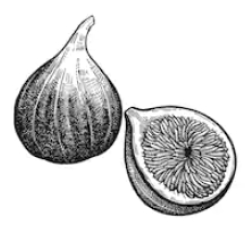
\includegraphics[width=1in,height=1.25in,clip,keepaspectratio]{fig1}}]{Michael Shell}
% Use $\backslash${\tt{begin\{IEEEbiography\}}} and then for the 1st argument use $\backslash${\tt{includegraphics}} to declare and link the author photo.
% Use the author name as the 3rd argument followed by the biography text.
% \end{IEEEbiography}

\vspace{11pt}

\vfill

\end{document}
